\documentclass[fontsize=11pt]{article} 
\usepackage[spanish]{babel} 
\usepackage[total={6in, 8in}]{geometry}
\usepackage{amsmath,amsfonts,amsthm} 
\usepackage{graphicx}
\graphicspath{ {images/} }
\usepackage{hyperref}
\usepackage[utf8]{inputenc}
\title{Proyecto Demografía Matemática}
\author{  López Hernández Alejandro $|$ Montoya Franco Luis Angel} % Your name
\date{\normalsize\today} % Today's date or a custom date
\begin{document}
\begin{titlepage}
	\centering
	
\includegraphics[width=0.15\textwidth]{UNAM}\par\vspace{1cm}
	{\scshape\LARGE Universidad Nacional Autónoma de México\par}
	\vspace{1cm}
	{\scshape\Large Facultad de Estudios Superiores Acatlán\par}
	\vspace{1.5cm}
	{\huge\bfseries Estudio demográfico de Chihuahua y consecuencias de los homicidios  \par}
	\vspace{2cm}
	{\scshape\Large Demografía Matemática\par}
	\vspace{2cm}
	{\Large\itshape López Hernández Alejandro \\ Montoya Franco Luis Angel\par}
	\vfill
	Profesor\par
	Ramos López Aram Isai

	\vfill

% Bottom of the page
	{\large \today\par}
\end{titlepage}
\begin{abstract}
   El objetivo de este proyecto es usar datos poblacionales del estado de Chihauhua para analizarlos y a partir del analisis poder corregirlos y estudiar la estructura poblacional, posteriormente usando las defunciones durante el año 2015 en Chihuahua causadas por agresiones, estimar el efecto que tienen sobre nuestra población ($_u AV_{j}$). 
\end{abstract}

\section*{Introducción}
En el estado de Chihuahua se tiene una de las ciudades con mayor violencia en el país, como es Ciudad Juarez, donde en particular se tiene una gran cantidad de feminicidios. Chihuahua es también interesante debido a su extensión territorial. 
\\ 
\section*{Distribución de la población por grupos etarios}
\section*{Desegregacion y preferencia al declarar edades}
\section*{Impacto de los homicidios en la esperanza de vida}
Como bien se sabe se tiene un gran problema de homicidios en el estado de Chihuahua, durante el año 2015 se reportaron\cite{DAT} los siguientes homicidios: 


\begin{table}[h!]
\centering

\begin{tabular}{|c|c|c|}
\hline
Edad  & Hombres & Mujeres \\ \hline
0     & 2       & 1       \\ \hline
1-4   & 8       & 2       \\ \hline
5-9   & 4       & 2       \\ \hline
10-14 & 11      & 6       \\ \hline
15-19 & 136     & 9       \\ \hline
20-24 & 213     & 20      \\ \hline
25-29 & 227     & 26      \\ \hline
30-34 & 173     & 19      \\ \hline
35-39 & 185     & 14      \\ \hline
40-44 & 162     & 19      \\ \hline
45-49 & 102     & 6       \\ \hline
50-54 & 61      & 3       \\ \hline
55-59 & 38      & 7       \\ \hline
60-64 & 28      & 2       \\ \hline
65-69 & 17      & 3       \\ \hline
70-74 & 13      & 1       \\ \hline
75-79 & 10      & 1       \\ \hline
80-84 & 5       & 1       \\ \hline
\end{tabular}
\caption{Muertes por agresiones en Chihuahua durante 2015}
\end{table}
\label{my-label}
Estos homicidios principalmente ocurrieron en Ciudad Juarez como muestra el siguiente mapa 
\begin{center}
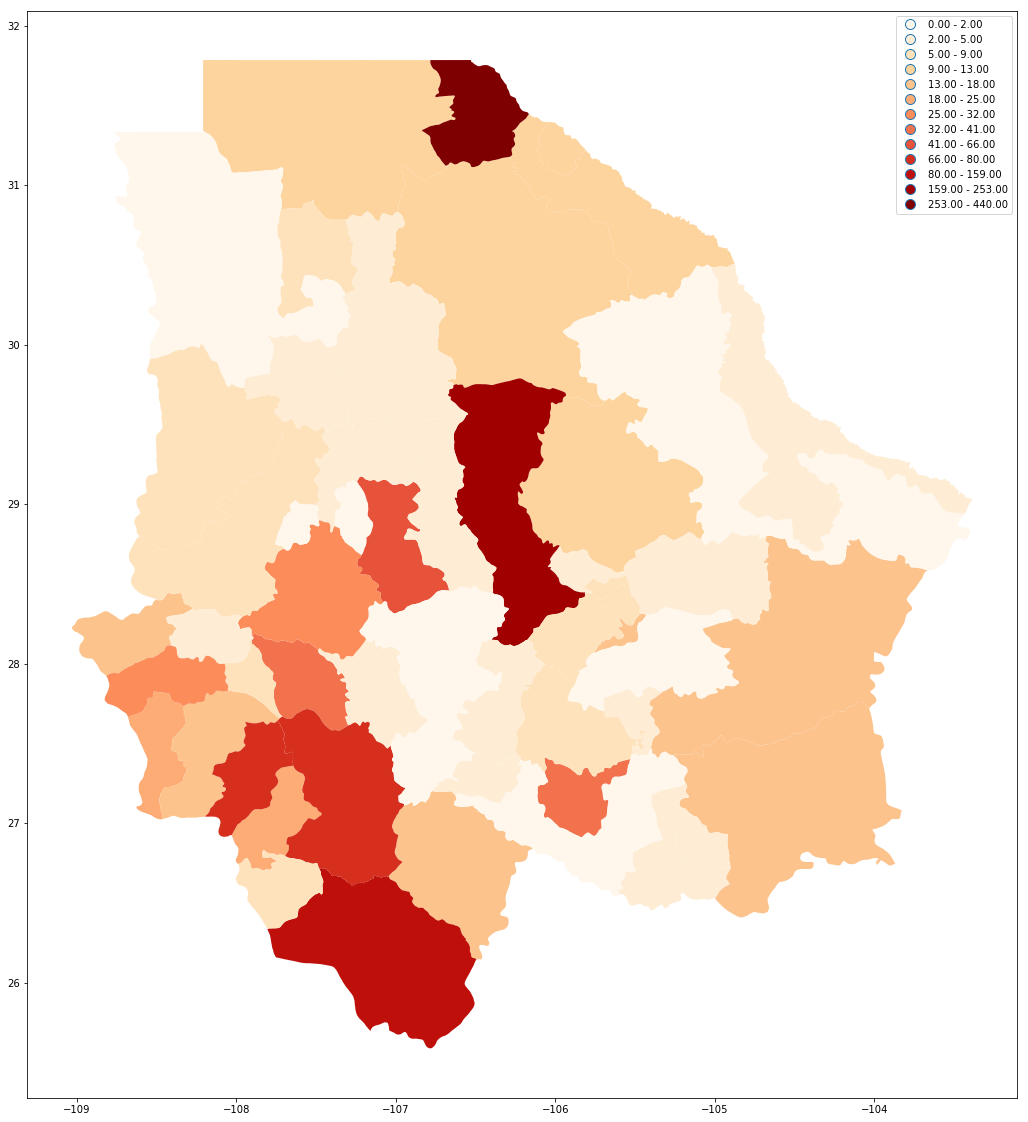
\includegraphics[width=0.6\textwidth]{map}
\end{center}
\section*{Conclusiones}
\begin{thebibliography}{X}
\bibitem{CAS} \textsc{Jacob S. Siegel} y \textsc{David A. Swanson}, \textit{The Methods And
Materials Of Demography}, Segunda edición,
Elsevier Academic Press, USA, 2004.
\bibitem{ARR} \textit{Eduardo E. Arriaga}\textit{ Los Años Vida Perdidos: Su Utilización Para Medir El Nivel y Cambio de la Mortalidad} , \textsc{U.S. Bureau of the Census} 
\bibitem{DAT} Defunciones registradas durante el año 2015 (Consultado el 29 de Octubre de 2017)  \url{https://datos.gob.mx/busca/dataset/estadistica-de-defunciones-registradas/resource/c346a78b-d91c-431c-8d2b-2f0831d3163c} Consultado el 29 de Octubre de 2017 
\bibitem{INE} Datos poblacionales de la encuesta intercensal 2015 (Consultado el 29 de Octubre de 2017 ) \url{http://www.beta.inegi.org.mx/proyectos/enchogares/especiales/intercensal/} 
\bibitem{CON} Proyecciones de población de la CONAPO (Consultado el 31 de Octubre de 2017) \url{http://www.conapo.gob.mx/es/CONAPO/Proyecciones} 
\bibitem{REP} Repositorio en GitHub con todos los procedimientos usados en este documento \url{https://github.com/aleespa/Demografia}
\end{thebibliography}

\end{document}